\newpage
\subsection{考察}
まず,外皮アリ・ナシで尾びれの振りに差が出てしまったことについて考察する.原因としては外皮に作った溝が胴体の屈曲を阻害し,本来胴体が屈曲するはずだった
位置まで動くことができなかったと考えられる(図\ref{fig:sogai}).実際に外皮を装着した状態で空中で振幅を測定してみる.測定した結果,プーリの回転角が$30\:^\circ$,
$45\:^\circ$,$60\:^\circ$のとき,尾ビレ振幅はそれぞれ$81\:^\circ$,$88\:^\circ$,$128\:^\circ$となった.本来の尾びれ振幅$81\:^\circ$,
$114\:^\circ$,$168\:^\circ$と比較すると約$40\:^\circ$差があるのがわかる(表\ref{tb:amp}).しかしここで外皮ナシと外皮アリで角度が比較的近い$81\:^\circ$と
$88\:^\circ$で比較しても実験結果と同じように外皮装着時のほうが速度が速くなっているので実験結果に影響を与えてしまうものではないと考える.
さらに言えば外皮アリの時の尾びれ振幅を実際の角度に近づけて実験を行えば,今回の結果よりもより優れた遊泳性能を示す実験結果を得ることができるといえる.

次に遊泳時に進行方向が傾いたことについて考察する.昨年度卒業研究ではワイヤーが左右に偏ることによって進行方向が傾いていたため,今回の実験では,ワイヤーの張力が左右に
偏ることを防ぐために,サーボモータの基準角度を変更してワイヤーの張力が偏らないようにプログラムを組んでいた.しかし,基準角をプログラムで調整しても進行方向が少し傾いて
しまったり,遊泳実験をしている最中に今まで直進していた設定の時に進行方向が曲がってしまうことがあった.
原因として考えられることは2つある.1つ目は外皮を装着することによって胴体を屈曲させるためのトルクが増大し,
\begin{table}[htbp]
    \centering
    \caption{サーボ巻き取り角と尾びれ振幅の関係}
    \label{tb:amp}
    \begin{tabular}{|c||c|c|}\hline
        サーボ巻き取り角[deg]&実験で使用した振幅[deg]&外皮装着時の振幅[deg]\\ \hline
        30&81&n\\ \hline
        45&114&88\\ \hline
        60&168&128\\ \hline
    \end{tabular}
\end{table}
\begin{figure}[hb]
    \centering
    \begin{tabular}{cc}
        \begin{minipage}[b]{0.4\linewidth}
            \centering
            \setPicture{gaihi_jama_nasi.png}
            \subcaption{外皮未装着時の胴体屈曲状態}
            \label{fig:jama_nasi}
        \end{minipage}
        \hspace{0.1\linewidth}
        \begin{minipage}[b]{0.4\linewidth}
            \centering
            \setPicture{gaihi_jama.png}
            \subcaption{外皮装着時の胴体屈曲状態}
            \label{fig:jama}
        \end{minipage}
    \end{tabular}
    \caption{外皮による屈曲の阻害}
    \label{fig:sogai}
\end{figure}
それに伴って糸が伸びた,またはたるんでしまったということが考えられる.
2つ目はスタート時の姿勢が若干左右どちらかに傾いてしまったことにより,結果として左右に進行方向が傾いているように見えたと考えられる.
改善策として,糸の張力を一定にできる治具をロボットに取り付ける,もしくは使用するワイヤを現在使用しているワイヤよりも強度が高いものにするといったことがあげられる.

次に外皮ナシの状態の時に振幅の変化によってそこまで速度にそこまで大きな変化が無かったことについて考察する.外皮無しで振幅$168\:^\circ$,周波数1.75 Hz時の遊泳時
の様子を見てみると(図\ref{fig:teikou})推進時に体が大きく屈曲してしまい,進行方向からの抵抗力を頭部と胴体部の一部で受けてしまっていることが分かる.これによっ
て本来その振幅で得られるはずだった推進力が低減し,遊泳速度が振幅によって変化しなかったと考えられる.
\begin{figure}[t]
    \centering
    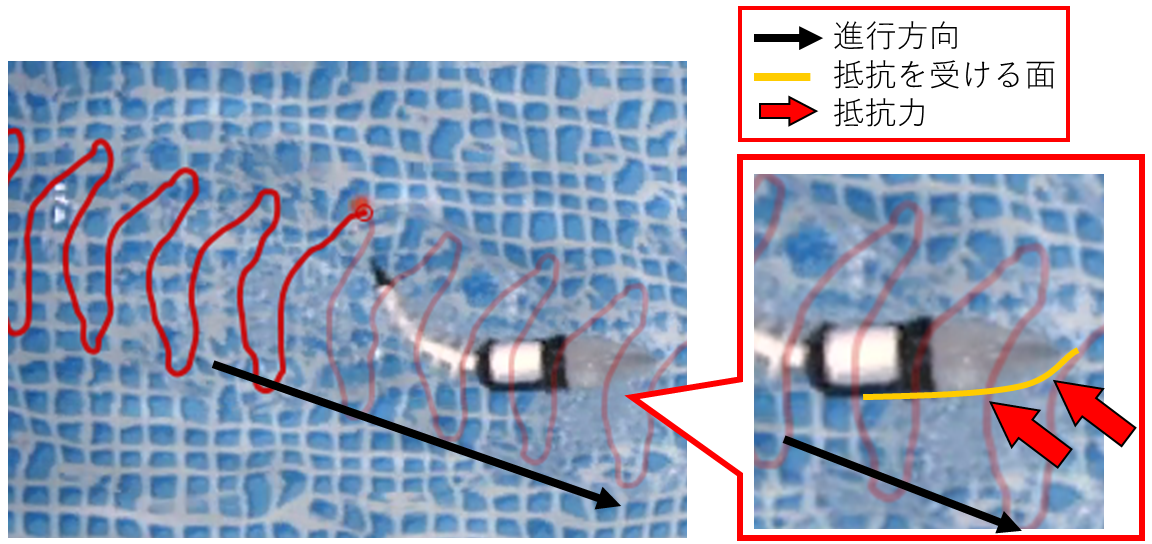
\includegraphics[width=0.9\linewidth]{chapters/picture/teikou.png}
    \caption{外皮未装着時に受ける抵抗}
    \label{fig:teikou}
\end{figure}
\begin{figure}[t]
    \centering
    \begin{tabular}{cc}
        \begin{minipage}[b]{0.45\linewidth}
            \centering
            \setPicture{compare_withoutskin.eps}
            \subcaption{外皮未装着時}
            \label{fig:without_matome}
        \end{minipage}
        \begin{minipage}[b]{0.45\linewidth}
            \centering
            \setPicture{compare_withskin.eps}
            \subcaption{外皮装着時}
            \label{fig:withskin_matome}
        \end{minipage}
    \end{tabular}
    \caption{外皮未装着時・装着時の結果をまとめたグラフ}
    \label{fig:matome}
\end{figure}
次に高周波数域において外皮が遊泳性能に与える影響について考察する.図\ref{fig:matome}に外皮有り・無しそれぞれの結果を一つのグラフにまとめたものを示す.グラフから低周波数域において
は外皮有り・無し両方において振幅による速度の変化はそれほど大きくは無かった.しかし,高周波数域を見てみると,外皮未装着時では振幅によってそこまで遊泳速度に差がない
のに対し,外皮装着時は振幅が大きくなるほど遊泳速度に差が出ていることが分かる.このことから高周波数域において柔軟外皮は遊泳性能に大きな影響を与えると考えられる.

\begin{figure}[t]
    \centering
    \setPicture{body.pdf}
    \caption{外皮の有無によるボディの違い}
    \label{fig:body}
\end{figure}

最後に外皮を装着することによってなぜ遊泳速度が向上したのかについて考察する.要因として考えられるのは外皮装着時と未装着時でボディが異なっていることである.外皮未装着時のボディは半流
線型のボディになっているのに対し,外皮装着時は流線型のボディになっている(図\ref{fig:body}).ここで流線型のボディはほかの形状に比べて物体の正面と背面の圧力差によって生じる圧力抵抗を低減することができ
る.したがって,ロボットのボディを流線型にすることによって水中で受ける抵抗力が減り,その分推進力が増大したと考えられる.
このことから,魚型ロボットに流線型のボディを備えることは遊泳性能の向上につながるといえる.